\documentclass{beamer}
\usepackage[utf8]{inputenc}
\usepackage[english, russian]{babel}
\usepackage[T1, T2A]{fontenc}
\usepackage{tabu}
\setbeamertemplate{footline}[frame number]
\setbeamertemplate{headline}{}
\usepackage{graphicx}
\graphicspath{ {stepen'.png}{graf.png}{hromate.png}{raskraska.png}{g.png}{g1.png}{g2.png}{g3.png}{Greedy.png}{kod.png}{polnyi.png}{color_tabl.png}}

\title{Раскраска графа}
\author{Шамакова Екатерина}
\institute{shamaich0168@gmail.com}
\thispagestyle{empty}
\date{}

\begin{document}

	\frame {
		\titlepage
	}
	\frame {
		\frametitle{План:}
\begin{itemize}
\item Что такое граф и основные определения, связанные с ним
\item Постановка задачи
\item Алгоритмы реализации раскаски графа
\begin{itemize}
\item Полный перебор
\item Жадный алгоритм
\end{itemize}
\item Инструкция пользователя
\item Выводы
\end{itemize}
	}
	\frame{
		\frametitle{Основные определения}
Графом называют математическую модель, представляющую собой множество вершин и набор рёбер

Вершины: { 1, 2, 3, 4, 5, 6, 7, 8}

Рёбра: 1-2,	 1-5,	 2-3,	 3-4,	 5-4	  ...
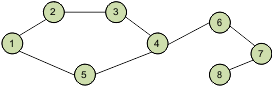
\includegraphics{graf} 

Две вершины считаются \textbf{\textit{смежными}}, если имеют хотя бы одно общее ребро
 }
	\frame{
		 \frametitle{Основные определения}
	  \begin{figure}
  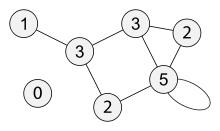
\includegraphics{stepen'}
\caption{Граф, на вершинах которого отмечены степени}
\end{figure}

\textbf{\textit{Степень}} или \textbf{\textit{валентность}} вершины графа — это число ребер, входящих в эту вершину. 
	}
\frame{
		 \frametitle{Основные определения}
Наименьшее число красок, необходимое для правильной раскраски графа G называется\textbf{\textit{хроматическим числом}}  графа G. Хроматическое число обозначается через $\chi(G)$.
  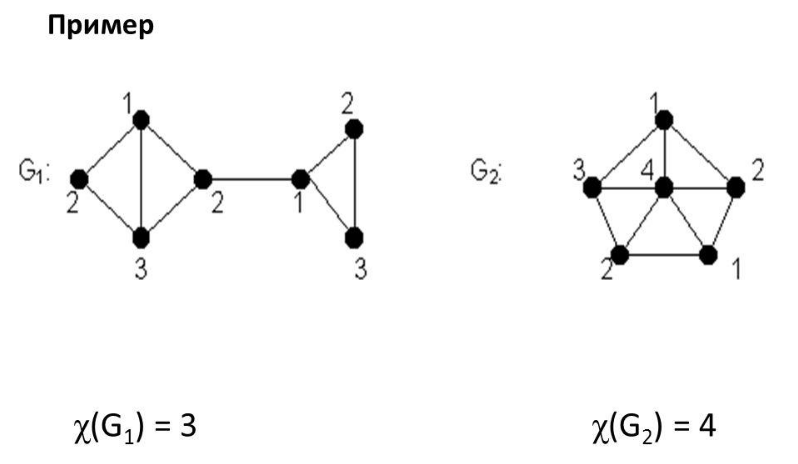
\includegraphics[scale=0.5]{hromate}

	}
\frame{
		 \frametitle{Раскраска графа}
	 \begin{itemize}
\item Раскрасить вершины графа
\item Любые 2 смежные вершины имеют разные цвета
\item Используя минимальное количество цветов
\end{itemize}
 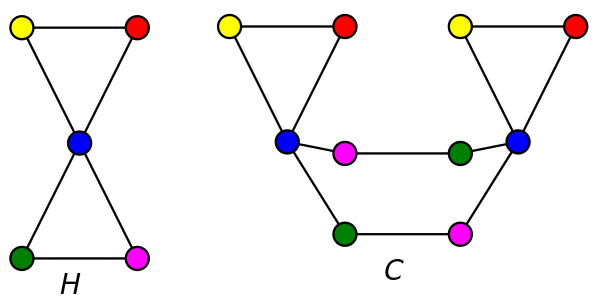
\includegraphics[scale=0.5]{raskraska}

	}
\frame{
		 \frametitle{Алгоритмы раскраски графа}
	 \begin{itemize}
\item Полный перебор
\item Жадный алгоритм
\end{itemize}
	}
\frame{
		 \frametitle{Полный Перебор}
Рассматривает \(k^n\) комбинаций цветов в графе, где k -- количество цветов в графе( хроматическое число ), а n -- количество вершин графа

Затем проверяет каждый вариант на корректность

Сложность данного алгоритма в худшем случае составит О(\(n^n\))

\begin{figure}[!]
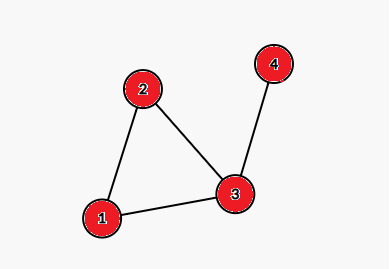
\includegraphics[scale=0.35]{g}
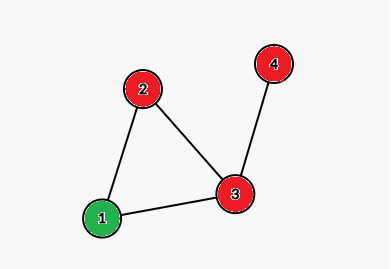
\includegraphics[scale=0.35]{g1}
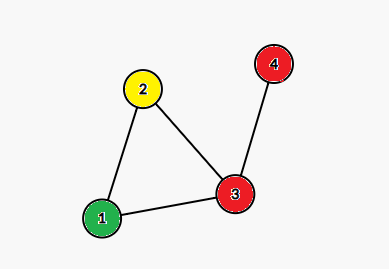
\includegraphics[scale=0.35]{g2}
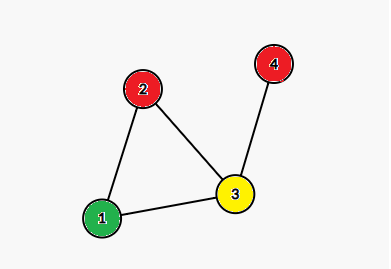
\includegraphics[scale=0.35]{g3}
\end{figure}
	
	}
\frame{
		 \frametitle{Полный Перебор ( псевдокод )}
	 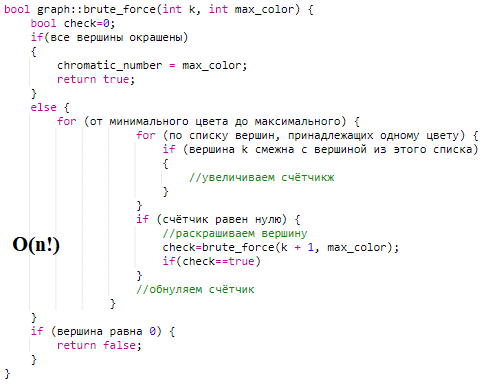
\includegraphics[scale=0.75]{polnyi}
	}
\frame{
		 \frametitle{Жадный алгоритм}
\begin{enumerate}
  \item Сортируем вершины по их степеням в порядке убывания
  \item  Последовательно окрашиваем вершины в выбранный цвет. Если у вершины уже есть смежная вершины с выбранный цветом, то оставляем ее неокрашенной.
 \item Если остались неокрашенные вершины, то выбираем следующий цвет и возвращемся ко 2 пункту
\end{enumerate}

Качество полученной раскраски зависит от выбранного порядка.Жадный не всегда даёт оптимальное решение.

Например:
	 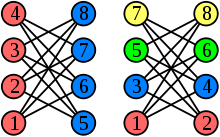
\includegraphics[scale=0.5]{Greedy}

	}
\frame{
		 \frametitle{Жадный алгоритм}
Способ хранения раскрашенных вершин: vector< list< int > > table



 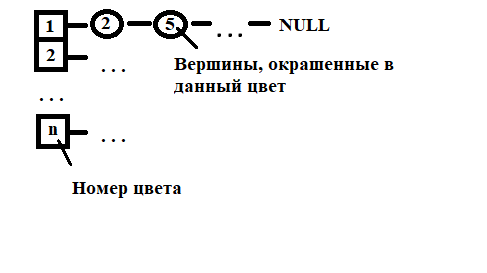
\includegraphics[scale=0.8]{color_tabl}
	}
\frame{
		 \frametitle{Жадный алгоритм ( псевдокод )}
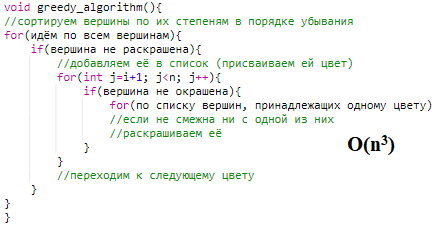
\includegraphics[width=12cm]{kod}
	}
\frame{
		 \frametitle{Инструкция пользователя}
Необходимо ввести: in.txt out.gv algNum
\begin{itemize}
\item in.txt: текстовый файл, в котором первой строкой записано количество вершин графа, а далее -- матрица смежности через пробел
\item out.gv: файл, в который запишется раскрашенный граф в формате graphviz
\item algNum: 0-полный перебор, 1-жадный алгоритм
\end{itemize}

Пример файла in.txt:

3

\begin{tabular}{c c c }
0 & 1 & 1 \\
1 & 0 & 1 \\
1 & 1 & 0
\end{tabular}

Далее в ходе выполнения программы необходимо будет ввести указанное количество цветов на английском языке через "Enter"
	}
\frame{
		 \frametitle{Вывод}
\begin{center}
\begin{tabu} to 1.0\textwidth { | X[l] | X[c] | X[r] | }
 \hline
 Название алгоритма & Сложность & Качество \\
 \hline
Жадный алгоритм  &  О(\(n^3\)) & есть контр. пример  \\
\hline
 Полный перебор  & О(\(n^n\))  & оптимальный  \\
\hline
\end{tabu}
\end{center}
	}
\end{document}